\documentclass[./main.tex]{subfiles}

\begin{document}
\onehalfspacing

\section{Ենթաբազմության ներքնամասը, անջատելիության $\textrm{T}_{0}$, $\textrm{T}_{1}$, $\textrm{T}_{2}$ աքսիոմները։ Մետրիկա, մետրիկական և մետրական տարածություններ։}\label{sec:7}

\par Ճիշտ այնպես, ինչպես բաց են\-թա\-բազ\-մութ\-յանը համարժեք այլընտ\-րանք է փակ ենթաբազմությունը, այդպես էլ ենթաբազմության փակմանը համարժեք այլընտ\-րանք է ենթաբազմության ներքնամաս հասկացությունը։ Ընդ որում, եթե ենթա\-բազմութ\-յան փակումը նրան պարունակող (որոշ իմաստով) «ամենափոքր» փակ ենթա\-բազ\-մութ\-յունն է, ապա են\-թա\-բազ\-մութ\-յան ներքնամասը նրա մեջ պարունակվող «ամենամեծ» բաց ենթաբազմու\-թյունն է։

\par Դիցուք $(X, \tau)$-ն տոպոլոգիական տարածություն է, $A$-ն $X$-ի որևէ ենթա\-բազմու\-թյուն է։

\begin{definition}
$x \in X$ կետը կոչվում է $A$ \textbf{ենթաբազմության ներքին կետ}, եթե գոյություն ունի $x$-ի $U_x$ շրջակայք, որ $x\in U_x \subset A$։ Տվյալ $A$ ենթաբազմության բոլոր ներքին կետերի բազմությունը կոչվում է $A$-ի \textbf{ներքնամաս} և նշանակվում է $\inter A$։
\end{definition}
\par Նկատենք, որ ներքին կետի սահմանման մեջ կարելի է պահանջել, որ $U_x$-ը լինի $x$ կետի բաց շրջակայք։ Այն, որ այդ երկու տարբերակները համարժեք են միմյանց, հետևում է կետի շրջակայքի սահմանումից (հիմնավորե՛լ)։
%\par \vspace{4.5pt} \textbf{Ներքնամասի հատկությունները․}
\paragraph*{Ներքնամասի հատկությունները․}
\begin{enumerate}
    \item $\inter A \subset A$ և $\inter A$-ն $X$-ի բաց ենթաբազմություն է։ Իրոք, $\inter A= \bigcup U_x$, որտեղ միավորումը կատարվում է ըստ բոլոր $x \in   \inter A$ կետերի։ Հետևաբար $\inter A$-ն բաց ենթաբազմություն է որպես $U_x$ բաց ենթաբազմությունների միավորում։
    \item $\inter A$-ն $A$-ի մեջ պարունակվող բոլոր բաց ենթաբազմություններից ամենամեծն է հետևյալ իմաստով․ եթե $V$-ն $A$-ի որևէ բաց ենթաբազմություն է, ապա $V \subset  \inter A$։ Իրոք, $V$-ի բոլոր կետերը, լինելով ներքին կետեր $V$-ի համար, ներքին կետեր են նաև $A$-ի համար, ուստի $V \subset   \inter A$։
    \item $A \mapsto \inter A$ համադրումը գործողություն է որոշված $X$-ի բոլոր են\-թա\-բազ\-մութ\-յուն\-նե\-րի բազմության վրա։ Մասնավորապես $ \inter\varnothing=\varnothing,\ \inter X=X$։ Այդ գործողությունը բնութագրում է $X$-ի բաց ենթաբազմությունները հետևյալ ի\-մաս\-տով․ $X$-ի որևէ ենթաբազմություն բաց ենթաբազմություն է այն և միայն այն դեպքում, երբ այն համընկնում է իր ներքնամասի հետ։ Իրոք, եթե $A$-ն բաց ենթաբազմություն է, ապա $A=\inter A$ ըստ ներքնամասի սահմանման։ Հակառակը՝ եթե $A= \inter A$, ապա $A$-ն բաց ենթաբազմություն է ըստ հատ\-կութ\-յուն 1-ի։
\end{enumerate}

\begin{nexamples}
$(X,\textrm{դիսկր․})$ տարածությունում ցանկացած $A \subset X$ ենթաբազմութ\-յան ներքնամասը $A$-ն է։ Իսկ $(X, \textrm{անտիդ․})$-ում $\inter A=X$, երբ $A=X$, և $\inter A=\varnothing$, երբ $A \neq X$։ Այնուհետև, $(\R, \textrm{սովոր․})$ տարածությունում $(a,b),\ [a,b),\ (a,b],\ [a,b]$ ենթաբազմությունների ներքնամասը $(a,b)$-ն է, իսկ ամբողջ թվերի $\Z$, ռացիոնալ թվերի $\Q$, իռացիոնալ թվերի $I$ բազմությունների ներքնամասերը $\varnothing$ բազմությունն է, $(\R, \textrm{հաշվ․ լր․})$ տարածությունում $\inter \Z= \inter \Q=\varnothing$, իսկ $\inter I=I$։
\end{nexamples}
\paragraph*{Ներքնամասի հատկությունները \normalfont (շարունակություն)։}
% \textbf{Ներքնամասի հատկությունները} (շարունակություն)։
\begin{enumerate}
    \item [4.] 	Եթե $A \subset B \subset X$, ապա $\inter A \subset  \inter B$ (հետևում է սահմանումից)։ 
    \item [5.] 	Ցանկացած $A, B \subset X$ ենթաբազմությունների դեպքում $ \inter(A \cap B)=\inter A \cap  \inter B$։
    \par Իրոք, $A \cap B \subset A \ \Rightarrow\ \inter(A\cap B)\subset \inter A$։ Նման ձևով $\inter(A\cap B)\subset \inter B\ \Rightarrow\ \inter(A\cap B)\subset(\inter A)\cap( \inter B)$։ Հակառակը՝ 
    \begin{equation*}
    \begin{aligned}
    x\in(\inter A)\cap( \inter B) &\Rightarrow \begin{cases} x\in  \inter A \\ x\in \inter B\end{cases}\hspace{-1em}\ \Rightarrow\ \begin{cases} \exists U_x\in\tau,\textrm{ որ } x\in U_x\subset A\\ \exists V_x\in\tau,\textrm{ որ } x\in V_x\subset B\end{cases}\hspace{-1em}\ \Rightarrow \\ &\Rightarrow \begin{cases} (U_x\cap V_x)\in\tau \\ x\in (U_x\cap V_x)\subset A\cap B\end{cases}\hspace{-1em}\ \Rightarrow\ x\in \inter(A \cap B)։
    \end{aligned}
    \end{equation*}
    \item [6.] Ցանկացած $A,B\subset X$ ենթաբազմությունների դեպքում $(\inter A)\cup(\inter B)\subset \inter(A\cup B)$։
    \par Իրոք, $A \subset A \cup B,\ B \subset A \cup B \Rightarrow (\inter A,\ \inter B \subset \inter (A \cup B)) \Rightarrow(  \inter A) \cup (\inter B) \subset  \inter(A \cup B)$։ Նկատենք, որ ընդհանուր 
դեպքում $(\inter A) \cup (\inter B) \neq \inter(A \cup B)$։ Որպես օրինակ՝ $(\R,\textrm{ սովոր․})$-ում դիտարկենք
$A=\Q$ և $B=I$ ենթաբազմությունները։ Մի կողմից՝ $\inter \Q= \inter I= \varnothing \Rightarrow \inter \Q 
\cup \inter I=\varnothing$, իսկ մյուս կողմից $\inter(\Q \cup I)= \inter \R=\R$։
\end{enumerate}
\subsection*{Անջատելիության աքսիոմները տոպոլոգիական տարածություններում}

\par Անջատելիության աքսիոմները լուծում են հետևյալ խնդիրը․ եթե տվյալ տո\-պո\-լո\-գիա\-կան տարածությունում ունենք երկու կետեր կամ (ընդհանուր դեպքում) երկու ենթաբազմություններ, հնարավո՞ր է արդյոք դրանք մասնակիորեն կամ լիովին տար\-ան\-ջատել միմյանցից չհատվող շրջակայքերով։ Ստորև կքննարկենք երկու կե\-տե\-րի տարանջատման խնդիրը երեք տարբերակով ($\textrm{T}_0$, $\textrm{T}_1$, $\textrm{T}_2$ աքսիոմներ)։


\begin{definition} Ասում են, որ $X$ տոպոլոգիական տարածությունը բավարարում է \textbf{անջատելիության $\boldsymbol{\textrm{T}}_0$ աքսիոմին} (կարճ՝ $X$-ը $\textrm{T}_0$ տարածություն է), եթե $X$-ի կամայական երկու տարբեր կետերից գոնե մեկն ունի շրջակայք, որը չի պարունակում մյուս կետը։
\end{definition}

\par Նկատենք, որ ոչ բոլոր տարածություններն են բավարարում այդ պայմանին․ այդպիսի օրինակ է երկուսից ոչ պակաս կետերով $(X, \textrm{անտիդ․})$-ը (հիմնավորե՛լ)։

\begin{definition} Ասում են, որ $X$ տոպոլոգիական տարածությունը բավարարում է \textbf{անջատելիության $\boldsymbol{\textrm{T}}_1$ աքսիոմին}, եթե նրա $\forall x_1 \neq x_2$ կետերից յուրաքանչյուրն ունի շրջակայք, որը չի պարունակում մյուս կետը։
\end{definition}

\par Պարզ է, որ $\textrm{T}_1$ աքսիոմին բավարարող տարածությունը բավարարում է նաև $\textrm{T}_0$ աքսիոմին։ Հակառակը ճիշտ չէ․ $X=\{ x_1,x_2 \}$ բազմությունը $\tau_1= \{\varnothing, \{x_1\}, \{x_1,x_2\}\}$ տոպոլոգիայով $\textrm{T}_0$ տարածություն է, բայց $\textrm{T}_1$ տարածություն չէ (ինչո՞ւ)։

\begin{definition} Ասում են, որ $X$ տոպ․ տարածությունը \textbf{$\boldsymbol{\textrm{T}}_2$} (կամ \textbf{հաուսդորֆյան}) \textbf{տարածություն} է, եթե նրա $\forall x_1 \neq x_2$ կետեր ունեն չհատվող շրջակայքեր։
\end{definition} 
$\textrm{T}_2$ տարածության պարզագույն օրինակ է որևէ երկկետանոց բազմություն դիսկ\-րետ տոպոլոգիայով։
\par Պարզ է, որ $\textrm{T}_2$ աքսիոմին բավարարող ամեն մի տարածություն բավարարում է նաև $\textrm{T}_1$-ին։ Հակառակը ճիշտ չէ․ օրինակ կբերենք քիչ հետո։ Իսկ հիմա․

\begin{theorem} $X$ տոպոլոգիական տարածությունը $\textrm{T}_1$ տարածություն է այն և միայն այն դեպքում, երբ նրա յուրաքանչյուր մի կետանոց $\{x\}$ ենթաբազմություն փակ ենթաբազմություն է։
\end{theorem} 

\begin{proof} \textbf{Պայմանի անհրաժեշտությունը։} Դիցուք $X$-ը $\textrm{T}_1$ տարածություն է, ցույց տանք, որ $\forall x \in X$ կետի դեպքում $X \setminus \{x\}$ ենթաբազմությունը բաց են\-թա\-բազ\-մութ\-յուն է, որից կհետևի, որ $\{x\}$-ը փակ է։ Դիտարկենք $\forall y \in X \setminus \{x\}$ կետ։ Ըստ պայմանի՝ գոյություն ունի $y$ կետի $U_y$ շրջակայք, որ $x \notin U_y$։  Նշանակում է $U_y \subset X \setminus \{x\}$։ Այսպիսով $X \setminus \{x\}$-ը շրջակայք է իր ամեն մի կետի համար $\Rightarrow X \setminus \{x\}\textrm{-ը}$ բաց ենթաբազմություն է։ \textbf{Պայմանի բավարարությունը։} Ունենք, որ $\forall \{x\} \subset X$ ենթաբազմություն փակ ենթաբազմություն է։ Կամայական $x_1 \neq x_2$ կետերի համար $X \setminus \{x_2\}$-ը և $X \setminus \{x_1\}$-ը համապատասխանաբար $x_1$-ի և $x_2$-ի բաց շրջակայքեր են, ընդ որում՝ $x_1 \notin X \setminus \{x_1\}$ և $x_2 \notin X \setminus \{x_2\}$։
\end{proof}

\par Այժմ բերենք $\textrm{T}_1$ տարածության օրինակ, որը $\textrm{T}_2$ տարածություն չէ։ Դիտարկենք որևէ $(X,\textrm{վերջ․ լր․})$ տարածություն, որտեղ $X$-ը անվերջ բազմություն է։ Սա $\textrm{T}_1$ տարածություն է (քանի որ ցանկացած մի կետանոց ենթաբազմություն փակ ենթաբազմություն է), բայց $\textrm{T}_2$ տարածություն չէ, քանի որ այս տարածությունում ցանկացած երկու բաց ենթաբազմություններ ունեն ոչ դատարկ հատում (հիմ\-նա\-վո\-րե՛լ)։

\paragraph*{Մետրիկական և մետրական տարածություններ։}
%\par \textbf{Մետրական տարածություններ։}
Սահմանվել են Մ․ Ֆրեշեի կող\-մից 1906 թվա\-կա\-նին։ Նպատակն է կամայական բազմություններում, ներմուծելով կետերի միջև հե\-ռա\-վո\-րու\-թյան հասկացություն, զարգացնել երկրաչափությանը և անալիզին բնորոշ ամենաընդհանուր և խորքային առանձնահատկություններով տե\-սություն։

\par Դիցուք $X$-ը որևէ բազմություն է, $\R$-ը թվային ուղիղն է։

\begin{definition} $\rho:X \times X \rightarrow \R$ որևէ արտապատկերում կոչվում է \textbf{մետրիկա} $X$ \textbf{բազմու\-թյան վրա}, եթե կամայական $x,y,z \in X$ տարրերի դեպքում բավարարվում են հետևյալ երեք պայմանները․
\begin{enumerate}
    \item $\rho(x,y)=0 \Leftrightarrow x=y$ (նույնականացման աքսիոմ),
    \item $\rho(x,y)=\rho(y,x)$ (համաչափության աքսիոմ),
    \item $\rho(x,z) \leq \rho(x,y)+\rho(y,z)$ (եռանկյան աքսիոմ)։
\end{enumerate}
\end{definition}

\begin{hetevanqax}
Վերցնելով 3-ում $z=x$՝ ստանում ենք $\rho(x,y) \geq 0$, $\forall x,y \in X$ տարրերի դեպքում։ Այժմ տեսնում ենք, որ բազմության վրա մետրիկան տարրական երկրաչափությունից հայտնի կետերի միջև հեռավորության ընդհանրա\-ցումն է կա\-մա\-յա\-կան բազմությունների դեպքում։
\end{hetevanqax}

\begin{definition} $(X,\rho)$ զույգը (այսինքն $X$ բազմությունը՝ իր վրա տրված $\rho$ մետ\-րի\-կա\-յով) կոչվում է \textbf{մետրիկական տարածություն}, իսկ $\rho(x,y)$ թիվը՝ $x$ և $y$ \textbf{կետերի միջև հե\-ռա\-վո\-րութ\-յուն} տվյալ մետրիկական տարածությունում։
\end{definition}

\begin{example} \label{օրինակ 1}
Ցանկացած $X$ բազմություն կարելի է վերածել մետ\-րիկա\-կան տա\-րա\-ծութ\-յան առնվազն մի եղանակով՝ $\rho(x,y)=1$, երբ $x \neq y$ և $\rho(x,y)=0$, երբ $x=y$։ Այս մետրիկական տարածությունը կոչվում է \textbf{դիսկրետ մետրիկական տարածություն} (անվանումը կպարզաբանվի մի փոքր ուշ)։
\end{example}


\begin{example} \label{օրինակ 2}
$\R$ թվային ուղղի վրա սահմանենք մետրիկա՝ $\rho(x,y)= \abs{x-y}$։ Այն կոչվում է թվային ուղղի \textbf{սովորական} կամ \textbf{էվկլիդյան մետրիկա}։
\end{example}


\par 1-3 աքսիոմների ստուգումը օրինակներ \hyperref[օրինակ 1]{1}, \hyperref[օրինակ 2]{2}-ում թողնվում է ընթերցողին որպես օգտակար խնդիր։ Հաջորդ կարևոր օրինակը ընդհանրացնում է \hyperref[օրինակ 2]{օրինակ 2}-ի էվկլիդ\-յան մետրիկան։

\begin{example}
Դիտարկենք $n$ չափականության $\R^n$ կոորդինատային տարածությունը և սահմանենք $x=(x_1,\dots,x_n )$, $y=(y_1,\dots,y_n)$ կետերի միջև հեռավորություն $\rho(x,y)=\sqrt{(x_1-y_1)^2+ \dots +(x_n-y_n)^2}$ բանաձևով։ 3-րդ աքսիոմը (սովորաբար դժվարություն է այս աքսիոմի ստուգումը) հետևում է Կոշի-Բունյակովսկու ան\-հա\-վա\-սա\-րու\-թյու\-նից․
\[ \sum_{k=1}^n a_k b_k \leq \sqrt{\sum_{k=1}^n a_k^2}\cdot \sqrt{\sum_{k=1}^n b_k^2}
\]
թվերի կամայական $(a_1,a_2,\dots,a_n)$ և $b_1, b_2, \dots, b_n$ հաջորդականությունների դեպքում։
\par Իրոք, $\forall x,y,z \in \R^n$ կետերի համար 3-րդ աքսիոմն ընդունում է 
\[\sqrt{\sum_{k=1}^n (x_k-z_k)^2}\leq \sqrt{\sum_{k=1}^n (x_k-y_k)^2} +\sqrt{\sum_{k=1}^n (y_k-z_k)^2}
\]
տեսքը։ Նշանակելով $x_k-y_k=a_k,\ y_k-z_k=b_k$ ստանում ենք՝ $x_k-z_k=a_k+b_k$, և 3-րդ աքսիոմն ընդունում է նոր՝ $\sqrt{\sum\limits_k (a_k+b_k)^2} \leq \sqrt{\sum\limits_k a_k^2} + \sqrt{\sum\limits_k b_k^2}$ տեսք։ Այն համարժեք է ${\sum\limits_k a_k \cdot b_k \leq \sqrt{\sum\limits_k a_k^2}} \cdot {\sqrt{\sum\limits_k b_k^2}}$ անհավասարությանը։ Այսպիսով մնում է ապացուցել Կոշի-Բունյակովսկու անհավասարությունը։

\par Արվում է դա այսպես․ կամայական $t \in \R$ դեպքում ունենք $\sum\limits_k \left(a_k-t\cdot b_k\right)^2 \geq 0$, որը կարելի է գրել $\left(\sum\limits_k b_k^2\right) t^2-2\left(\sum\limits_k a_k b_k\right)t+\left(\sum\limits_k a_k^2 \right) \geq 0$ տեսքով։ Սրանից հետևում է $\left(\sum\limits_k a_k b_k\right)^2 \leq \left(\sum\limits_k a_k^2\right)\cdot\left(\sum\limits_k b_k^2\right)$ անհավասարությունը, որից էլ ստանում ենք $\sum\limits_k a_k b_k \leq \sqrt{\sum\limits_k a_k^2} \cdot \sqrt{\sum\limits_k b_k^2}$։ \qed

\par Եթե $\rho$-ն մետրիկա է $X$ բազմության վրա, ապա ցանկացած $c>0$ թվի դեպքում $c\rho$-ն (սահմանվում է $(c\rho)(x,y)=c\cdot\rho(x,y)$ բանաձևով) ակնհայտորեն նույնպես մետրիկա է $X$-ի վրա։ Մետրիկա է նաև $\widebar{\rho} = \dfrac{\rho}{1+\rho}$ արտապատկերումը՝ սահմանված $\widebar{\rho}(x,y) = \dfrac{\rho(x,y)}{1+\rho(x,y)}$ բանաձևով։ Ստուգենք 3-րդ աքսիոմը $\widebar{\rho}$-ի համար։ Նախ նկատենք, որ

\begin{center}
$\widebar{\rho}(x,z) = \dfrac{\rho(x,z)}{1+\rho(x,z)} \leq \dfrac{\rho(x,y) + \rho(y,z)}{1+\rho(x,y) + \rho(y,z)}$
\end{center}
(ստուգվում է անմիջականորեն՝ ազատվելով հայտարարներից)։ Այնուհետև
\begin{equation*}
    \begin{aligned}
    \widebar{\rho}(x,z) &\leq \dfrac{\rho(x,y)}{1+\rho(x,y) + \rho(y,z)} +  \dfrac{\rho(y,z)}{1 + \rho(x,y) + \rho(y,z)} \leq  \dfrac{\rho(x,y)}{1+\rho(x,y)} + \dfrac{\rho(y,z)}{1+\rho(y,z)} =\\ &= \widebar{\rho}(x,y) + \widebar{\rho}(y,z)
    \end{aligned}
\end{equation*}

\par Նշենք, որ ստացված $(X, \widebar{\rho})$ մետրական տարածությունում $\widebar{\rho}(x,y) < 1,\ \forall x,y \in X$ կետերի դեպքում։
\end{example}

% +
\begin{definition}
Երկու $(x_1, \rho_1)$ և $(x_2, \rho_2)$ մետրիկական տարածություններ կոչվում են \textbf{իզոմետրիկ տարածություններ}, եթե գոյություն ունի $\varphi : X_1 \rightarrow X_2$ բիյեկտիվ ար\-տա\-պատ\-կե\-րում, որ $\rho_1(x,y) = \rho_2(\varphi(x), \varphi(y)),\ \forall x, y \in X$ կետերի դեպքում։
\end{definition}

\par Հեշտ է տեսնել, որ $X = \R$ թվային ուղղի վրա օրինակներ\hyperref[1]{1}-ում և \hyperref[2]{2}-ում սահման\-ված մետրիկաներից ստացվող մետրիկական տա\-րա\-ծու\-թյուն\-ները իզոմետրիկ տա\-րա\-ծութ\-յուն\-ներ չեն (ինչո՞ւ)։
\par Իզոմետրիկ չեն նաև $(X, \rho)$ և $(X, \widebar{\rho})$ մետրիկական տարածությունները, եթե թեկուզ մի զույգ $x,y \in X$ կետերի դեպքում $\rho(x,y)\geq 1$։
\par Իսկ ահա \hyperref[օրինակ 1]{օրինակ 1}-ում վերցնելով մի դեպքում $X = \Q$, իսկ մյուս դեպքում՝ $X = \Z$, ստանում ենք իզոմետրիկ տարածություններ (հիմնավորե՛լ)։

\begin{definition}
    Դիցուք $(X, \rho)$-ն որևէ մետրիկական տարածություն է, $a\in X, r>0$։
    Հետևյալ ենթաբազմությունները՝ $\mathcal{D}(a, r) = \{x\in X\mid \rho(a, x) < r\},\ \mathcal{B}(a, r) = \{x\in X\mid \rho(a, x) \leq r\},\ \mathcal{S}(a, r) = \{x\in X\mid \rho(a, x) = r\}$ կոչվում են $(X,\rho)$-ի հա\-մա\-պա\-տաս\-խա\-նա\-բար $a$ կենտրոնով և $r$ շառավղով \textbf{անեզր գունդ, եզրով գունդ և սֆերա}։
    \par Այս անվանումները մեկնաբանելու համար նշենք, որ $\mathcal{B}(a, r)$ և $\mathcal{D}(a, r)$ գնդերի համար եզր է $\mathcal{S}(a, r)$ սֆերան։ Պարզ է, որ $\mathcal{B}(a, r)$ գունդը պարունակում է իր եզրը, իսկ $\mathcal{D}(a, r)$ գունդը՝ ոչ։
\end{definition}

\begin{nexamples}
        ա) Դիսկրետ  $(X,\rho)$ մետրիկական տարածությունում
        \par $\mathcal{D}(a, r) = \mathcal{B}(a, r) = \{a\}$ և $\mathcal{S}(a, r) = \varnothing$ երբ $r<1$,
        \par $\mathcal{D}(a, r) = \mathcal{B}(a, r) = X$ և $\mathcal{S}(a, r) = \varnothing$ երբ $r>1$,
        \par $\mathcal{D}(a, 1) = \{a\},\ \mathcal{B}(a, 1) = X,\ \mathcal{S}(a, 1) = X \setminus \{a\}$։
        \par բ) $\R^n$ մետրիկական (կոորդինատային) տարածությունում՝\par
        $n=1$ դեպքում ունենք՝ $\mathcal{D}(a, r) =(a-r,a+r),\  \mathcal{B}(a, r) =[a-r,a+r],\ \mathcal{S}(a, r) = \{a-r, a+r\}$։\par
        $n=2$ դեպքում ունենք՝ $\mathcal{D}(a, r) = \{(x_1,x_2)\mid x_1^2+x_2^2 < r^2\}$ անեզր շրջան, $\mathcal{B}(a, r) =  \{(x_1,x_2)\mid x_1^2+x_2^2 \leq r^2\}$ եզրով շրջան, $\mathcal{S}(a, r) = \{(x_1,x_2)\mid x_1^2+x_2^2 = r^2\}$ շրջանագիծ:\par
        $n=3$ դեպքում ունենք՝ $\mathcal{D}(a, r) = \{(x_1,x_2,x_3)\mid x_1^2+x_2^2+x_3^2 < r^2\}$ անեզր գունդ, $\mathcal{B}(a, r) =  \{(x_1,x_2,x_3)\mid x_1^2+x_2^2+x_3^2 \leq r^2\}$ եզրով գունդ և $\mathcal{S}(a, r) =  \{(x_1,x_2,x_3)\mid x_1^2+x_2^2+x_3^2 = r^2\}$ գնդային մակերևույթ այդ տերմինների սովորական իմաստով։
\end{nexamples}

\begin{theorem}
$(X,\rho)$ մետրիկական տարածության բոլոր $\mathcal{D}(a,r)$ անեզր գնդերի բազ\-մութ\-յունը հանդիսանում է բազա $X$-ի ինչ-որ տոպոլոգիայի համար (այդ տոպոլոգիան կոչվում է $X$-ի \textbf{մետրական տոպոլոգիա}, որի մասին ասում են, որ այն ծնված է $X$-ի $\rho$ մետրիկայով)։
\end{theorem}
\label{թեորեմ 2}
\renewcommand*{\proofname}{\hspace{18pt}\textbf{Ապացուցման}\nopunct}
\begin{proof} հիմքում ընկած է \red{թեմա 5-ի թեորեմ 2}-ը, ըստ որի պետք է ստուգենք երկու պայման։

\begin{enumerate}
    \item [1.] $\bigcup \mathcal{D}(a,r)=X$ (հետևում է նրանից, որ միշտ $a \in \mathcal{D}(a,r))$։
    \item [2.] Ամեն մի ոչ դատարկ $\mathcal{D}(a,r_1 ) \cap \mathcal{D}(b,r_2)$ հատում ներկայացվում է որպես անեզր գնդերի միավորում։ Բավական է ցույց տալ, որ ցանկացած $x \in \mathcal{D}(a,r_1) \cap \mathcal{D}(b,r_2)$ կետի համար գոյություն ունի $\mathcal{D}(x,r)$ գունդ, որ $\mathcal{D}(x,r) \subset \mathcal{D}(a,r_1) \cap \mathcal{D}(b,r_2)$։ Այդ գնդի $r$ շառավղի մեծությունը որոշելու համար դիտարկենք մաս\-նա\-վոր դեպք․ որպես $(X, \rho)$ մետրիկական տարածություն վերցնենք $\R^2$ հար\-թութ\-յունը սովորական էվկլիդյան մետրիկայով։
\end{enumerate}
\begin{center}
\includegraphics[scale=0.7]{images/id12.png}
\end{center}
\par Ունենք՝ $\rho(a,x)<r_1,\rho(b,x)<r_2$։ Գծագրից երևում է․ եթե $r$-ը այնպիսին է, որ
\[
\begin{cases}
    \mathcal{D}(x,r) \subset D(a,r_1)\\
    \mathcal{D}(x,r) \subset D(b,r_2)
\end{cases}\hspace{-1em},
\textrm{ ապա }
\begin{cases}
       \rho(a,x) + r \leq r_1\\
       \rho(b,x)+r \leq r_2
\end{cases} \hspace{-1em}\ \Rightarrow\
\begin{cases}
    r \leq r_1 - \rho(a,x)\\
    r \leq r_2 - \rho(b,x)
\end{cases}
\]

\par Ուստի, ընդհանուր դեպքում որպես $\mathcal{D}(x,r)$ գնդի որոնելի շառավիղ վերցնենք $r=\min⁡(r_1-\rho(a,x),{r_2-
\rho(b,x))}$ թիվը։ Այժմ դիտարկենք $\forall y\in \mathcal{D}(x,r)$ կետ և ցույց տանք, որ $y\in \mathcal{D}(a,r_1 
)\cap \mathcal{D}(b,r_2)$։ Դրա\-նից կհետևի, որ $x\in \mathcal{D}(x,r)\subset \mathcal{D}(a,r_1 )\cap 
\mathcal{D}(b,r_2)$։ \par
Կարող ենք գնահատել՝ $\rho(a,y)\leq \rho
(a,x)+\rho(x,y)<\rho(a,x)+r\leq \rho(a,x)+r_1-\rho
(a,x)=r_1$, ուստի $y\in \mathcal{D}(a,r_1)$։ Նման ձևով ստանում ենք $y\in \mathcal{D}(b,r_2)$, ուստի $y\in \mathcal{D}(a,r_1)\cap \mathcal{D}(b,r_2)$։
\end{proof}
\begin{note}
Ապացույցի ընթացքում $\mathcal{D}(x,r)$ գնդի $r$ շառավղի մեծությունը որոշվեց տեսողաբար, մասնավոր օրինակի միջոցով։ Անդրադառնալով ապացույցի մանրամասներին՝ նշենք, որ ամենասկզբում օգտվեցինք հետևյալ հուշումից․ եթե $\mathcal{D}(x,r)\subset \mathcal{D}(a,r_1)$, ապա $\rho(a,x)+r\leq r_1$։ Այլ, ավելի ընդհանուր ձևակերպումով դա հնչում է այսպես․ եթե մետրիկական տարածությունում մի գունդ ընկած է մեկ այլ գնդի մեջ, ապա առաջին գնդի շառավիղը փոքր կամ հավասար է երկրորդ գնդի շառավղից։ Բոլոր փորձերը սա դարձնել թեորեմ (դուրս բերել մետրիկայի աքսիոմներից) դատա\-պարտ\-ված են անհաջողության, քանի որ իրողությունն այլ է․ գոյություն ունեն մետրիկական տարածություններ, որոնցում փոքր շառավղով գունդն իր մեջ կարող է ներառել ավելի մեծ շառավղով գունդ (ընթերցողը կարող է ծանոթանալ այդպիսի օրինակի հետ Б. Гелбаум, Дж. Олмстед, Контрпримеры в анализе, 1967г. գրքում)։ Արժեզրկվո՞ւմ է արդյոք սրանով թեորեմ 2-ի վերը բերված ապացույցը։ Սկզբունքորեն ոչ, քանի որ ձևականորեն ապացույցն անթեր է։ Բայց հոգեբանորեն ինչ-որ տեղ՝ գուցե։ Թերևս սա է պատճառը, որ А.Н. Колмо\-го\-ров, С.В. Фомин, Элементы теории функции и функционального анализа դա\-սա\-գրքի երկրորդ գլխում հեղինակները գերադասել են մետրիկական տարածություն\-ներում նույն տոպոլոգիան սահմանել այլ եղանակով (խուսափելով $\mathcal{D}(x,r)$ գնդի շառավղի ընտրությունից), հիմնվելով Կուրատովսկու փակման գործողության վրա։ Կարծում ենք ընթերցողին հետաքրքիր և օգտակար կլինի ծանոթանալ նաև այդ եղանակի հետ։
\end{note}

\renewcommand*{\proofname}{\hspace{18pt}\textbf{Ապացուցում։}\nopunct}
\par Որպես հետևանք \hyperref[թեորեմ 2]{թեորեմ 2}-ից ստանում ենք, որ անեզր գնդերը բաց բազ\-մութ\-յուն\-ներ են տվյալ մետրական տոպոլոգիայում (այդ պատճառով կոչվում են նաև \textbf{բաց գնդեր})։ Ցույց տանք նաև, որ $\mathcal{B}(a,r)$ եզրով գնդերը փակ բազմություններ են մետ\-րա\-կան տոպոլոգիայում (այդ պատճառով կոչվում են նաև \textbf{փակ գնդեր})։ 



% \includegraphics[scale=0.4]{images/id13.png}
% 
\begin{center}
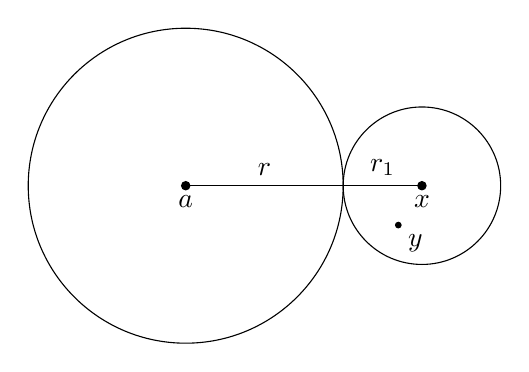
\begin{tikzpicture}
    % Draw circles
    \draw (0,0) circle (2cm);
    \draw (3,0) circle (1cm);

    % Draw radii
    \draw (0,0) -- (2,0) node[midway,above] {$r$};
    \draw (3,0) -- (2,0) node[midway,above] {$r_1$};

    % Add dots for the centers of the circles
    \filldraw[black] (0,0) circle (1.5pt);
    \filldraw[black] (3,0) circle (1.5pt);

    % Label centers
    \node at (0,-0.2) {$a$};
    \node at (3,-0.2) {$x$};

    % Adjust point y position higher
    \filldraw[black] (2.7,-0.5) circle (1pt) node[below right] {$y$};
\end{tikzpicture}
\end{center}

\par Դրա համար բավական է ապացուցել, որ $X\setminus \mathcal{B}(a,r)$ լրացումը շրջակայք է իր կամայական $x$ կետի համար, և հետևաբար բաց բազմություն է։ Սա հետևում է նրանից, որ $\mathcal{D}(x,r_1 )\subset X\setminus \mathcal{B}(a,r)$, որտեղ $r_1=\rho(a,x)-r$։ Իրոք, $\forall y\in \mathcal{D}(x,r_1)$ կետի համար
\[
    \rho(a,y)\geq \rho(a,x)-\rho(y,x)>\rho(a,x)-r_1=r, \textrm{ ուստի } \mathcal{D}(x,r_1) \subset X\setminus \mathcal{B}(a,r)։
\]

\par Նման ձևով ապացուցվում է, որ $\mathcal{S}(a,r)$ սֆերաները փակ բազմություններ են մետրական տոպոլոգիայում (հիմնավորե՛լ)։

\begin{theorem}
$(X,\rho)$ մետրիկական տարածության $A\subset X$ ենթաբազմությունը բաց է տվյալ մետրական տոպոլոգիայում այն և միայն այն դեպքում, երբ իր կամայական $a$ կետի հետ միասին պարունակում է $a$ կենտրոնով որևէ բաց գունդ։
\end{theorem}

\begin{center}
\includegraphics[scale=0.75]{images/id14.png}
\end{center}
\begin{proof}
Եթե $A$-ն բաց բազմություն է, ապա այն բաց գնդերի միավորում է ըստ \hyperref[թեորեմ 2]{թեորեմ 2}-ի։ Մնում է ցույց տալ, որ եթե $a$-ն պատկանում է որևէ $\mathcal{D}(b,r)$ բաց գնդի, ապա $\mathcal{D}(b,r)$-ն իր մեջ պարունակում է $a$ կենտրոնով որևէ բաց գունդ։
\par Վերցնենք $r'=r-\rho(a,b)$ և ցույց տանք, որ $\mathcal{D}(a,r')\subset \mathcal{D}(b,r)$։
Եթե $y\in \mathcal{D}(a,r')$, ապա $\rho(y,b)\leq \rho(y,a)+\rho(a,b)<r'+\rho(a,b)=r \Rightarrow y\in \mathcal{D}(b,r)$, ուստի $\mathcal{D}(a,r')\subset \mathcal{D}(b,r)$։ Թեորեմի հակառակ պնդումն ակնհայտ է։
\end{proof}


\begin{definition} Միևնույն $X$ բազմության վրա տրված երկու մետրիկա կոչվում են \textbf{համարժեք}, եթե նրանցով ծնված մետրական տոպոլոգիաները նույնն են։
\end{definition}

\begin{example}
Ցույց տանք, որ նույն $X$-ի վրա $\rho$ և $\widebar{\rho} = \dfrac{\rho}{1+\rho}$ մետրիկաները համար\-ժեք են (չնայած նրան, որ ընդհանուր դեպքում $(X,\rho)$ և $(X,\widebar{\rho})$ մետրիկական տարա\-ծու\-թյուն\-ները իզոմետրիկ չեն)։ Իրոք, $(X,\rho)$ տարածության ամեն մի $\mathcal{D}(a,r)\subset X$ բաց գունդ կարող է դիտարկվել որպես $(X,\widebar{\rho})$ տարածության $\widebar{\mathcal{D}}(a,R)\subset X$ բաց գունդ, որտեղ $R=\dfrac{r}{1+r}$, և հակառակը՝ $(X,\widebar{\rho})$ տարածության ամեն մի $\widebar{\mathcal{D}}(a, R)$ գունդ, եթե $R<1$, կարող է դիտարկվել որպես $(X,\rho)$ տարածության $\mathcal{D}(a,r)$ գունդ, որտեղ $r=\dfrac{R}{1-R}$։ Պարզունակ ստուգումը թողնվում է ընթերցողին։
\end{example}

% +
\par Այս օրինակը ցույց է տալիս, որ մետրիկական տարածությունների տեսությունը, որպես տոպոլոգիական տարածությունների ուսումնասիրություն, էապես տար\-բեր\-վում է մետրիկական տարածությունների ուսումնասիրությունից՝ հիմնված ի\-զո\-մետ\-րի\-կու\-թյան հասկացության վրա, դիտելով այն որպես տարածությունների նույնա\-կա\-նաց\-ման միջոց։
\par Հաշվի առնելով այս հանգամանքը, մենք որոշ դեպքերում «մետրիկական տա\-րա\-ծու\-թյուն» բառակապակցության փոխարեն կգործածենք «մետրական տարածութ\-յուն» բառակապակցությունը, ի նկատի ունենալով բազմություն իր վրա տրված մետրական տոպոլոգիայով։
% +
\par Մետրական տարածություններն օժտված են կարևոր հատկությամբ՝ բավարարում են անջատելիության $\textrm{T}_2$ աքսիոմին։ Իրոք, եթե $x_1,x_2 \in X$ և $x_1\neq x_2$, ապա $\rho(x_1,x_2) \neq 0$, ուստի $D(x_1, \frac{1}
{2} \rho(x_1,x_2))$ և $D(x_2, \frac{1}{2} \rho(x_1,x_2))$ բաց գնդերը $x_1$ և $x_2$ կետերի չհատվող 
շրջակայքեր են (ապացուցումը կատարվում է եռանկյան աքսիոմի միջոցով՝ թողնելով ընթերցողին)։

% +
\begin{definition}
Տոպոլոգիական տարածությունը կոչվում է \textbf{մետրացվող տա\-րա\-ծու\-թյուն}, եթե նրա տոպոլոգիան ծնվում է որևէ մետրիկայով։
\end{definition}

% -- 
\begin{nexample}
Ցանկացած $(X,\textrm{դիսկր․})$ տարածություն մետրացվող տարածություն է, քանի որ նրա տոպոլոգիան համընկնում է $X$-ի վրա $\rho(x,y)= \begin{cases} 0, \text{ երբ } x=y \\ 1, \text{ երբ } x \neq y \end{cases}$ դիսկրետ մետրիկայով ծնված տոպոլոգիայի հետ։


%+
\par Իրոք, $\mathcal{D}(x,1)=\{x\},\ \forall x \in X$ կետի դեպքում, ուստի $X$-ի բոլոր մի կետանոց ենթաբազմությունները (հետևաբար և $X$-ի բոլոր ենթաբազմությունները) բաց բազ\-մութ\-յուն\-ներ են տվյալ մետրական տոպոլոգիայում։ 

%+
\par Մյուս կողմից չմետրացվող տարածության օրինակ է մեկից ավելի կետեր պա\-րու\-նա\-կող ամեն մի $\forall (X,\textrm{անտիդ․})$ տարածություն, քանի որ այն չի բավարարում ան\-ջա\-տե\-լի\-ու\-թյան $\textrm{T}_2$ աքսիոմին (ինչո՞ւ)։ 
\end{nexample} 
\end{document}